
\section{The Prosthetic Control System}

Having extracted features from the three EMG datasets of one movement for each of the four movements, the control system could be build in order to achieve online recognition of movements. The following sections will explain the implementation of the control system and how the achieved level of control was assessed for each subject. 

\subsection{Building the Control System} 

The implementation of the control system was divided into two parts. To achieve recognition of performed movement a classifier was trained, however, this only produces a recognition of a movement and does not reflect the intensity of which the movement is being performed with. Therefore, following the recognition of the performed movements a linear regression model was implemented to achieve proportional control. 

\subsubsection{Movement Classification}

Online classification of movements was accomplished by implementing a LDA classifier. As presented in \secref{patter} the classifier needed to be trained using data from each movement. Hence, the five features extracted for each of the 40 $\percent$, 50 $\percent$ and 70 $\percent$ fraction of the pMVC for one movement were assembled into one labeled matrix. The same was done for the three remaining movements. A fifth class was labeled rest and its matrix only contained the features from a single rest acquisition. These matrices were made for the data acquired from each of the eight channels in the MYB. All matrices were assembled into one training matrix with labels for each movement. Using the \textit{fitcdicsr}-function in MATLAB a LDA classifier was trained by feeding it the training matrix. Hereby, the classifier was trained in separating 5 classes using linear decision boundaries. During online use, the \textit{predict}-function was used to evaluate features from new input data in the classifier and decide which movement there was being performed.    


\subsubsection{Proportional control}  
When a movement was decided upon by the classifier, the proportional control provided the control system with an actual output to move the virtual prosthesis. For this purpose a multiple linear regression model was created for each of the four movements, through the MATLAB function \textit{fitlm}. The models were fitted with the MAV features extracted from the fraction of pMVC data as well as the mean of the pMVC data. The data was scaled such that the pMVC data was set to 1 and the remaining data was scaled in relation to that. In the online control, the output of the decided regression models was written such that it would move in the direction described in \secref{sec:vp}. The output from the regression models was limited to a maximum of 1, meaning that maximum level of activation detecting was the pMVC level.  Another threshold implemented was a minimum activation of at least 15 $\percent$ for a movement to count, otherwise no output would be provided. This idea behind this implementation was to provide a more stable resting state in addition to the classifier. 


\subsection{Assessment of Subject Control}

After the acquisition of data training data and the training of the classifier, two stages where the subject could familiarize themselves with the control and test how well they were able to use the control system, were implemented. It was highly critical that the subject was able to achieve sufficient control abilities such that it would not be due to poor control that a subject was not able to reach a target during test of the feedback schemes. However, as the classifier only had five classes, representing five separable movements to distinguish between, a robust online control was achieved in an evaluation test during pilot tests after short training trials. Therefore, the need for subject training could be kept to a minimum.  

\subsubsection{Familiarization with Control}

At first, the subject was presented with an image of the grid, which can be seen in \figref{fig:meth:gridmap}, in \secref{sec:vp}. The subject was able to control a cursor and navigate around inside the grid by performing supination to go right, pronation to go left, open and closed hand to go up and down, and rest to stand still. The familiarization was separated into two stages. In the first stage, the user had three minutes to get acquainted the functionality of the control moving the cursor shown in \figref{fig:C1} (a). The cursor acted as a direct output of the control. During the three minute familiarization, the subject was instructed in training unflawed performance of each movement and the transition from a movement to rest. In the second stage, the visual feedback in the form of the cursor was made more discrete. This was done by making the cursor invisible and instead highlighting the outlines of the target that contained the cursor. This discretized cursor representation was included to make the visual feedback identical in resolution to the sensory feedback. The discrete visual feedback can be seen in \figref{fig:C1} (b). Again the subject had three minutes to familiarize with the control. 

\begin{figure}[H]
	\subfigure[Illustration of the cursor used during the first familiarization stage.]
	{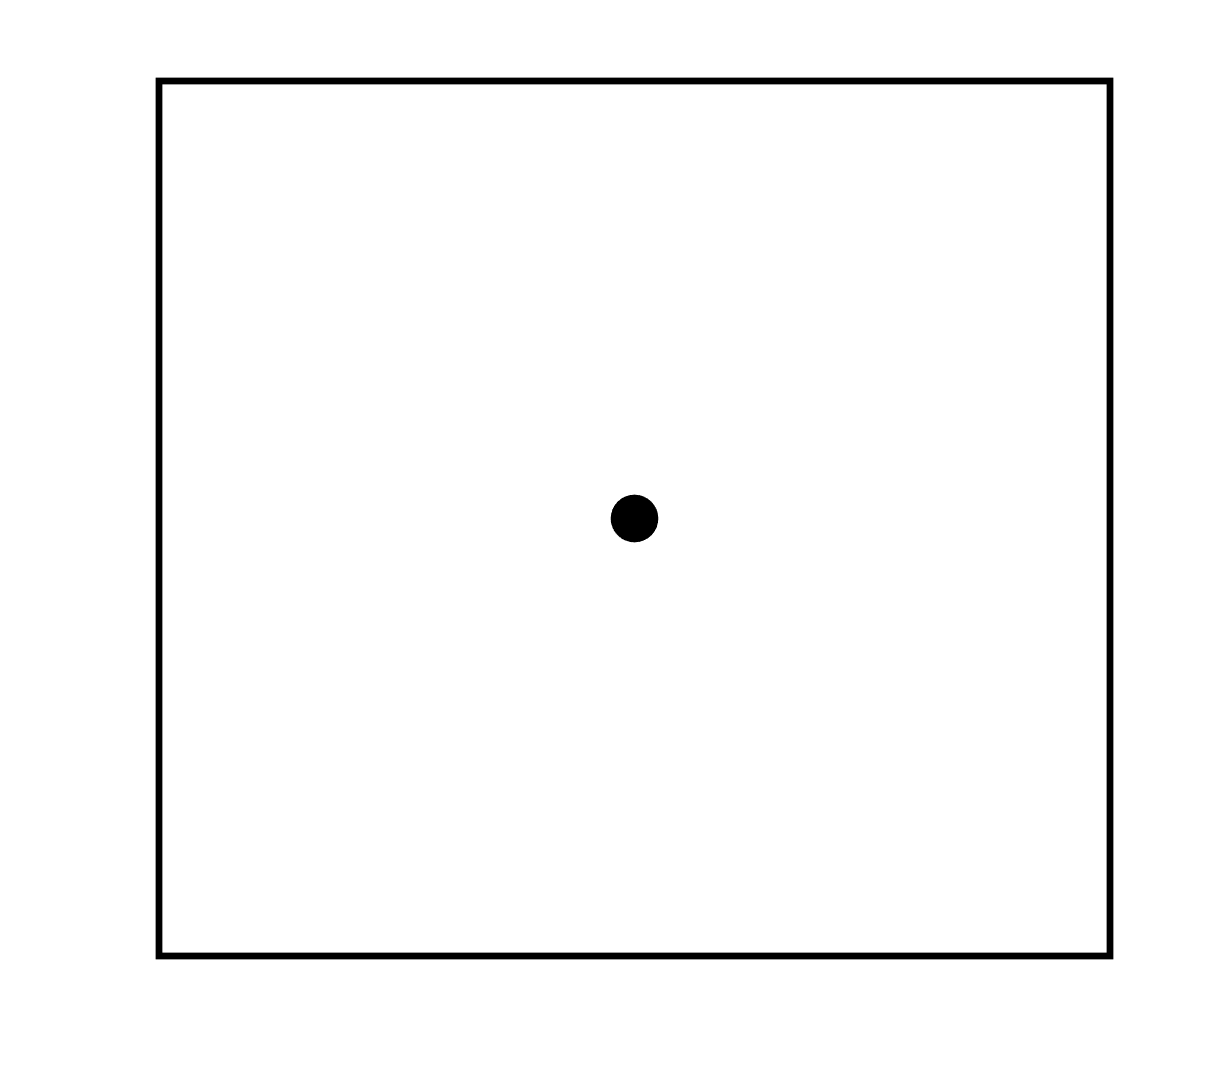
\includegraphics[width=0.34\textwidth]{figures/cursor}}
	\hspace{0.9cm}
	\subfigure[Illustration of the cursor used during the second familiarization stage. ]
	{
\includegraphics[width=0.34\textwidth]{figures/blue}}
	\caption{Illustration of the cursor used in the two stage familiarization with control.  Using this cursor in (a) the subject was informed the exact location of cursor in a square. Using this cursor in (b) the subject was provided with the information of which square the cursor was in, but not the exact location of the cursor inside the square. }
	\label{fig:C1}
\end{figure}

\subsubsection{Evaluation Test}

After completion of the two stages of familiarization, a target reaching test was carried out. In this test, a square was highlighted with red and the subject would have to move the discretized cursor to the desired target and dwell inside it for 1.5 seconds in order for it to be deemed reached. The subject had 30 seconds to reach a target. The test was designed such that each of the 24 squares in the grid was to be reached. When a target was either reached or the time to reach the target ran out, the cursor would be reset to the neutral position (first row, third column in \figref{fig:meth:gridmap}). \\
The target reaching test was made such that a measure of how well the subjects was able to use the control system could be obtained. Hereby it also acted as a reference for the later comparisons with control in combination with the two feedback schemes. Furthermore, if the investigators deemed the achieved subject control insufficient, the investigators could choose to exclude the subject.       













